\documentclass{wissdoc}
% Autor: Roland Bless 1996-2009, bless <at> kit.edu
% ----------------------------------------------------------------
% Diplomarbeit - Hauptdokument
% ----------------------------------------------------------------
%%
%% $Id: thesis.tex 65 2012-05-10 10:32:11Z bless $
%%
% wissdoc Optionen: draft, relaxed, pdf --> siehe wissdoc.cls
% ------------------------------------------------------------------
% Weitere packages: (Dokumentation dazu durch "latex <package>.dtx")
\usepackage[numbers,sort&compress]{natbib}
% \usepackage{varioref}
% \usepackage{verbatim}
% \usepackage{float}    %z.B. \floatstyle{ruled}\restylefloat{figure}
% \usepackage{subfigure}
% \usepackage{fancybox} % für schattierte,ovale Boxen etc.
% \usepackage{tabularx} % automatische Spaltenbreite
% \usepackage{supertab} % mehrseitige Tabellen
% \usepackage[svnon,svnfoot]{svnver} % SVN Versionsinformation 
%% ---------------- end of usepackages -------------

%\svnversion{$Id: thesis.tex 65 2012-05-10 10:32:11Z bless $} % In case that you want to include version information in the footer

%% Informationen für die PDF-Datei
\hypersetup{
 pdfauthor={Chi Trung.Nguyen.},
 pdftitle={Speicherkomponenten eines PC}
 pdfsubject={Not set},
 pdfkeywords={Not set}
}

% Macros, nicht unbedingt notwendig
%%%%%%%%%%%%%%%%%%%%%%%%%%%%%%%%%%%%%%%%%%%%%%%%%%%%%%%%%%
% macros.tex -- einige mehr oder weniger nuetzliche Makros
% Autor: Roland Bless 1998
%%%%%%%%%%%%%%%%%%%%%%%%%%%%%%%%%%%%%%%%%%%%%%%%%%%%%%%%%%
% $Id: macros.tex 33 2007-01-23 09:00:59Z bless $
%%%%%%%%%%%%%%%%%%%%%%%%%%%%%%%%%%%%%%%%%%%%%%%%%%%%%%%%%%


%%%%%%%%%%%%%%%%%%%%%%%
% Kommentare 
%%%%%%%%%%%%%%%%%%%%%%%
\ifnotdraftelse{
\newcommand{\Kommentar}[1]{}
}{\newcommand{\Kommentar}[1]{{\em #1}}}
% Alles innerhalb von \Hide{} oder \ignore{} 
% wird von LaTeX komplett ignoriert (wie ein Kommentar)
\newcommand{\Hide}[1]{}
\let\ignore\Hide

%%%%%%%%%%%%%%%%%%%%%%%%%
% Leere Seite ohne Seitennummer, wird aber gezaehlt
%%%%%%%%%%%%%%%%%%%%%%%%%

\newcommand{\leereseite}{% Leerseite ohne Seitennummer, nächste Seite rechts (wenn 2-seitig)
 \clearpage{\pagestyle{empty}\cleardoublepage}
}
%%%%%%%%%%%%%%%%%%%%%%%%%%
% Flattersatz rechts und Silbentrennung, Leerraum nach rechts maximal 1cm
%%%%%%%%%%%%%%%%%%%%%%%%%%
\makeatletter
\newcommand{\myraggedright}{%
 \let\\\@centercr\@rightskip 0pt plus 1cm
 \rightskip\@rightskip
  \leftskip\z@skip
  \parindent\z@
  \spaceskip=.3333em
  \xspaceskip=.5em}
\makeatother

\makeatletter
\newcommand{\mynewline}{%
 \@centercr\@rightskip 0pt plus 1cm
}
\makeatother


%%%%%%%%%%%%%%%%%%%%%%%%%%
% Für Index
%%%%%%%%%%%%%%%%%%%%%%%%%%
\makeatletter
\def\mydotfill{\leavevmode\xleaders\hb@xt@ .44em{\hss.\hss}\hfill\kern\z@}
\makeatother
\def\bold#1{{\bfseries #1}}
\newbox\dbox \setbox\dbox=\hbox to .4em{\hss.\hss} % dot box for leaders
\newskip\rrskipb \rrskipb=.5em plus3em % ragged right space before break
\newskip\rrskipa \rrskipa=-.17em plus -3em minus.11em % ditto, after
\newskip\rlskipa \rlskipa=0pt plus3em % ragged left space after break
\newskip\rlskipb \rlskipb=.33em plus-3em minus.11em % ragged left before break
\newskip\lskip \lskip=3.3\wd\dbox plus1fil minus.3\wd\dbox % for leaders
\newskip \lskipa \lskipa=-2.67em plus -3em minus.11em %after leaders
\mathchardef\rlpen=1000 \mathchardef\leadpen=600
\def\rrspace{\nobreak\hskip\rrskipb\penalty0\hskip\rrskipa}
\def\rlspace{\penalty\rlpen\hskip\rlskipb\vadjust{}\nobreak\hskip\rlskipa}
\let\indexbreak\rlspace
\def\raggedurl{\penalty10000 \hskip.5em plus15em \penalty0 \hskip-.17em plus-15em minus.11em}
\def\raggeditems{\nobreak\hskip\rrskipb \penalty\leadpen \hskip\rrskipa %
\vadjust{}\nobreak\leaders\copy\dbox\hskip\lskip %
\kern3em \penalty\leadpen \hskip\lskipa %
\vadjust{}\nobreak\hskip\rlskipa}
\renewcommand*\see[2]{\rlspace\emph{\seename}~#1} % from makeidx.sty

%%%%%%%%%%%%%%%%%%%%%%%%%%
% Neue Seite rechts, leere linke Seite ohne Headings
%%%%%%%%%%%%%%%%%%%%%%%%%%
\newcommand{\xcleardoublepage}
{{\pagestyle{empty}\cleardoublepage}}

%%%%%%%%%%%%%%%%%%%%%%%%%%
% Tabellenspaltentypen (benoetigt colortbl)
%%%%%%%%%%%%%%%%%%%%%%%%%%
\newcommand{\PBS}[1]{\let\temp=\\#1\let\\=\temp}
\newcolumntype{y}{>{\PBS{\raggedright\hspace{0pt}}}p{1.35cm}}
\newcolumntype{z}{>{\PBS{\raggedright\hspace{0pt}}}p{2.5cm}}
\newcolumntype{q}{>{\PBS{\raggedright\hspace{0pt}}}p{6.5cm}}
\newcolumntype{g}{>{\columncolor[gray]{0.8}}c} % Grau
\newcolumntype{G}{>{\columncolor[gray]{0.9}}c} % helleres Grau

%%%%%%%%%%%%%%%%%%%%%%%%%%
% Anführungszeichen oben und unten
%%%%%%%%%%%%%%%%%%%%%%%%%%
\newcommand{\anf}[1]{"`{#1}"'}

%%%%%%%%%%%%%%%%%%%%%%%%%%
% Tiefstellen von Text
%%%%%%%%%%%%%%%%%%%%%%%%%%
% S\tl{0} setzt die 0 unter das S (ohne Mathemodus!)
% zum Hochstellen gibt es uebrigens \textsuperscript
\makeatletter
\DeclareRobustCommand*\textlowerscript[1]{%
  \@textlowerscript{\selectfont#1}}
\def\@textlowerscript#1{%
  {\m@th\ensuremath{_{\mbox{\fontsize\sf@size\z@#1}}}}}
\let\tl\textlowerscript
\let\ts\textsuperscript
\makeatother

%%%%%%%%%%%%%%%%%%%%%%%%%%
% Gauß-Klammern
%%%%%%%%%%%%%%%%%%%%%%%%%%
\newcommand{\ceil}[1]{\lceil{#1}\rceil}
\newcommand{\floor}[1]{\lfloor{#1}\rfloor}

%%%%%%%%%%%%%%%%%%%%%%%%%%
% Average Operator (analog zu min, max)
%%%%%%%%%%%%%%%%%%%%%%%%%%
\def\avg{\mathop{\mathgroup\symoperators avg}}

%%%%%%%%%%%%%%%%%%%%%%%%%%
% Wortabkürzungen
%%%%%%%%%%%%%%%%%%%%%%%%%%
\def\zB{z.\,B.\ }
\def\dh{d.\,h.\ }
\def\ua{u.\,a.\ }
\def\su{s.\,u.\ }
\newcommand{\bzw}{bzw.\ }

%%%%%%%%%%%%%%%%%%%%%%%%%%%%%%%%%%%
% Einbinden von Graphiken
%%%%%%%%%%%%%%%%%%%%%%%%%%%%%%%%%%%
% global scaling factor
\def\gsf{0.9}
%% Graphik, 
%% 3 Argumente: Datei, Label, Unterschrift
\newcommand{\Abbildung}[3]{%
\begin{figure}[tbh] %
\centerline{\scalebox{\gsf}{\includegraphics*{#1}}} %
\caption{#3} %
\label{#2} %
\end{figure} %
}
\let\Abb\Abbildung
%% Abbps
%% Graphik, skaliert, Angabe der Position
%% 5 Argumente: Position, Breite (0 bis 1.0), Datei, Label, Unterschrift
\newcommand{\Abbildungps}[5]{%
\begin{figure}[#1]%
\begin{center}
\scalebox{\gsf}{\includegraphics*[width=#2\textwidth]{#3}}%
\caption{#5}%
\label{#4}%
\end{center}
\end{figure}%
}
\let\Abbps\Abbildungps
%% Graphik, Angabe der Position, frei wählbares Argument für includegraphics
%% 5 Argumente: Position, Optionen, Datei, Label, Unterschrift
\newcommand{\Abbildungpf}[5]{%
\begin{figure}[#1]%
\begin{center}
\scalebox{\gsf}{\includegraphics*[#2]{#3}}%
\caption{#5}%
\label{#4}%
\end{center}
\end{figure}%
}
\let\Abbpf\Abbildungpf

%%
% Anmerkung: \resizebox{x}{y}{box} skaliert die box auf Breite x und Höhe y,
%            ist x oder y ein !, dann wird das usprüngliche 
%            Seitenverhältnis beibehalten.
%            \rescalebox funktioniert ähnlich, nur das dort ein Faktor
%            statt einer Dimension angegeben wird.
%%
% \Abbps{Position}{Breite in Bruchteilen der Textbreite}{Dateiname}{Label}{Bildunterschrift}
%

\newcommand{\refAbb}[1]{%
s.~Abbildung \ref{#1}}

%%%%%%%%%%%%%%%%%%%%
%% end of macros.tex
%%%%%%%%%%%%%%%%%%%%

% Print URLs not in Typewriter Font
\def\UrlFont{\rm}

\newcommand{\blankpage}{% Leerseite ohne Seitennummer, nächste Seite rechts
 \clearpage{\pagestyle{empty}\cleardoublepage}
}

%% Einstellungen für das gesamte Dokument

% Trennhilfen
% Wichtig! 
% Im ngerman-paket sind zusätzlich folgende Trennhinweise enthalten:
% "- = zusätzliche Trennstelle
% "| = Vermeidung von Ligaturen und mögliche Trennung (bsp: Schaf"|fell)
% "~ = Bindestrich an dem keine Trennung erlaubt ist (bsp: bergauf und "~ab)
% "= = Bindestrich bei dem Worte vor und dahinter getrennt werden dürfen
% "" = Trennstelle ohne Erzeugung eines Trennstrichs (bsp: und/""oder)

% Trennhinweise fuer Woerter hier beschreiben
\hyphenation{
% Pro-to-koll-in-stan-zen
% Ma-na-ge-ment  Netz-werk-ele-men-ten
% Netz-werk Netz-werk-re-ser-vie-rung
% Netz-werk-adap-ter Fein-ju-stier-ung
% Da-ten-strom-spe-zi-fi-ka-tion Pa-ket-rumpf
% Kon-troll-in-stanz
}

% Index-Datei öffnen
\ifnotdraft{\makeindex}
%%%%%%%%%%%%%% includeonly %%%%%%%%%%%%%%%%%%%
% Es werden nur die Teile eingebunden, die hier 
% aufgefuehrt sind!
\includeonly{%
titelseite,%
erklaerung,% Ist in KA Pflicht für Diplomarbeiten
einleitung,% Motivation, Zielsetzung, Gliederung
%grundlagen,% Grundlagen 
nichttechnisch,
technisch,
%analyse,   % Problembeschreibung (Detail) und Related Work
%entwurf,   % Beschreibung der Problemlösung (Konzepte, allg. Architektur, ...)
%implemen,  % Beschreibung der Umsetzung/Implementierung
%eval,      % Nachweis und Auswertung
zusammenf  % Zusammenfassung der Ergebnisse und Ausblick
}
%%%%%%%%%%%%%%%%%%%%%%%%%%%%%%%%%%%%%%%%%%%%%%
\begin{document}

\frontmatter
\pagenumbering{roman}
\ifnotdraft{
 %% Titelseite
%% Vorlage $Id: titelseite.tex 61 2012-05-03 13:58:03Z bless $

\def\usesf{}
\let\usesf\sffamily % diese Zeile auskommentieren für normalen TeX Font

\newsavebox{\Erstgutachter}
\savebox{\Erstgutachter}{\usesf Prof.~Dr.~Jens Wagner}
\newsavebox{\Zweitgutachter}
\savebox{\Zweitgutachter}{\usesf Prof.~Dr.~?.~?????????}

\begin{titlepage}
\setlength{\unitlength}{1pt}
\begin{picture}(0,0)(85,770)

\includegraphics[width=\paperwidth]{logos/HFTL_Deckblatt}
\end{picture}

\thispagestyle{empty}

%\begin{titlepage}
%%\let\footnotesize\small \let\footnoterule\relax
\begin{center}
\hbox{}
\vfill
{\usesf
{\huge\bfseries Speicherkomponenten eines PC's\\
             \par}
\vskip 1.8cm
Studienarbeit\\
von\\[2mm]
\vskip 1cm

{\large\bfseries Chi Trung Nguyen\\}
\vskip 1.2cm
an der Hochschule für Telekommunikation Leipzig\\
in der Studienrichtung Wirtschaftsinformatik\\
%Universität Karlsruhe (TH)\\[2ex]
\vskip 3cm
\begin{tabular}{p{5.5cm}l}
Erstgutachter: & \usebox{\Erstgutachter} \\
\end{tabular}
\vskip 3cm
Bearbeitungszeit:\qquad 11.Juni~2012 -- 11.Juli~2012
}
\end{center}
\vfill
\end{titlepage}
%% Titelseite Ende


%%% Local Variables: 
%%% mode: latex
%%% TeX-master: "thesis"
%%% End: 

 %\blankpage % Leerseite auf Titelrückseite
 %
 % Die folgende Erklärung ist für Diplomarbeiten Pflicht
 % (siehe Prüfungsordnung), für Studienarbeiten nicht notwendig
 \thispagestyle{empty}
\vspace*{42\baselineskip}
\hbox to \textwidth{\hrulefill}
\par
Ich erkläre hiermit, dass ich die vorliegende Arbeit selbständig verfasst und
keine anderen als die angegebenen Quellen und Hilfsmittel verwendet habe.

München, den 11. Juli 2012

%%%%%%%%%%%%%%%%%%%%%%%%%%%%%%%%%%%%%%%%%%%%%%%%%%%%%%%%%%%%%%%%%%%%%%%%
%% Hinweis:
%%
%% Diese Erklärung wird von der Prüfungsordnung für Diplomarbeiten 
%% verlangt und ist zu unterschreiben. Für Studienarbeiten ist diese
%% Erklärung nicht zwingend notwendig, schadet aber auch nicht.
%%%%%%%%%%%%%%%%%%%%%%%%%%%%%%%%%%%%%%%%%%%%%%%%%%%%%%%%%%%%%%%%%%%%%%%%
\clearpage







 %\blankpage % Leerseite auf Erklärungsrückseite
}
%
%% *************** Hier geht's ab ****************
%% ++++++++++++++++++++++++++++++++++++++++++
%% Verzeichnisse
%% ++++++++++++++++++++++++++++++++++++++++++
\ifnotdraft{
{\parskip 0pt\tableofcontents} % toc bitte einzeilig
%\blankpage

%\blankpage
%\listoftables
%\blankpage
}


%% ++++++++++++++++++++++++++++++++++++++++++
%% Hauptteil
%% ++++++++++++++++++++++++++++++++++++++++++
\graphicspath{{Bilder/}}

\mainmatter
\pagenumbering{arabic}
%% Einleitung.tex
%% $Id: einleitung.tex 61 2012-05-03 13:58:03Z bless $
%%

\chapter{Einleitung}
\label{ch:Einleitung}
%% ==============================

In der digitalen Gesellschaft und im Zeitalter des Internets wird es immer wichtiger immer mehr Daten so schnell wie möglich zu speichern.  \textit{Ein Speicher (v. lat.: spicarium Getreidespeicher, aus spica Ähre)[...] ist ein Ort oder eine Einrichtung zum Einlagern von materiellen oder} \textbf{\textit{immateriellen}} \textit{Objekten.} \cite{wiki:Speicher}
\newline
Ein Speichermedium dient also zur kurz- oder langfristigen \glqq \textit{Einlagerung}\grqq{} bzw. Erhaltung von immateriellen Objekten – oder anders ausgedr"uckt Informationen. 
Es stellt sich die Frage: Was sind Informationen? \newline
Im Laufe der Geschichte wurde der Informationsbegriff immer wieder neu definiert. Für die Informatik ist die Beschreibung nach Claude Elwood Shannon\footnote[1]{Claude Elwood Shannon: * 30. April 1916 in Petoskey, Michigan; \textdagger{} 24. Februar in Melford, Massachusetts gilt als Begr"uender der Informationstheorie} relevant. Demnach muss man ein Zeichen als kleinste Informationseinheit und dessen statistische H"aufigkeit in einem Code als Information sehen. 
\newline
Die Information darf nicht mit dem Bedeutungsgehalt verwechselt werden. Eine Information die wenig Sinn ergibt ist einer Information mit großem Sinngehalt gleichwertig. Wichtiger zu betrachten ist die Wahrscheinlichkeit des Auftretens eines Zeichens im vorgegebenen Code. Je geringer diese ist, desto h"oher ist sein Informationsgehalt.
\\
Im wesentlichen werden Informationen auf Speichermedien aber in Form von Daten abgelegt. 
\\Mehrere aufeinanderfolgende Zeichen werden als Zeichenfolge bezeichnet.\cite{hansen:wi1}
\\ 
Daten sind nach ISO 2382 
\glqq \textit{Gebilde aus Zeichen oder kontinuierliche Funktionen, die aufgrund bekannter oder unterstellter Abmachungen Informationen darstellen, vorrangig zum Zweck der Verarbeitung und als deren Ergebnis.}\grqq{} 
\\
Somit sind nach einer bestimmten Syntax angeordneten Zeichen \textbf{Daten}.

%% ==============================
\section{Zielsetzung der Arbeit}
%% ==============================
\label{ch:Einleitung:sec:Zielsetzung}

Mit dieser Arbeit möchte ich auf grundlegende Prinzipien der Speicherung von Informationen auf verschiedenen Medien, insbesondere in der Informatik eingehen. Sie soll eine "Ubersicht auf M"oglichkeiten der Datenspeicherung im fr"uhen und heutigen Informationsalter schaffen und die Funktionsweise der Speichermedien erkl"aren. Auch wenn der Titel \glqq Speicherkomponenten eines PC \grqq{} ist, wird der Vollst"andigkeit halber trotzdem auf "altere, heute nicht mehr gebr"aubliche Wege Daten zu speichern R"ucksicht genommen. Der Leser sollte nach dem Lesen der Arbeit einen "Uberblick dar"uber haben, welche Methoden es gibt Informationen aufzubewahren. Es werden keine neuen wissenschaftlichen Erkenntnisse vorgestellt, sondern fachliche Informationen zusammengestellt.

%% ==============================
\section{Gliederung der Arbeit}
%% ==============================
\label{ch:Einleitung:sec:Gliederung}

Man unterscheidet zwischen technischer und nichttechnischer Speicherung. Die Speicherung von Informationen ist aber nicht einer Erfindung der Neuzeit. Seit jeher versucht der Mensch Informationen zu bewahren, damit diese nicht in Vergessenheit geraten. 
\\
So geh"oren auch H"ohlenmalereien dazu. Man sch"atzt, dass die "alteste H"ohlenmalerei etwa 40.000 Jahre alt ist. Bei dieser sogenannten nichttechnischen Speicherung ben"otigt es ein Tr"agermaterial wie Papier, Pergament, Papyrusrollen oder wie in diesem Beispiel Stein um Informationen zu erhalten. Ein gro"ser Nachteil kann jedoch die sp"atere Entzifferung der \glqq Daten\grqq{} sein, aber immerhin kann man diese sofort auslesen.
\\
Bei der technischen Speicherung bedarf es einer speziellen Methode um die gew"unschten Daten auszulesen. Diese sind nicht sofort per Auge oder mit der Hand erkennbar(vgl. Braille\footnote[2]{Braille: Schrift der Blinden. Die Schrift(verschiedene angeordnete Punkte) wird von Hinten auf Papier gepresst. Diese sind so mit den Fingern ertastbar}). 
%TODO: eingehen auf untere Kapitel(elektronische,magnetische speicherung etc
\\
Die Arbeit ist dementsprechend in diese beiden Teile strukturiert, wobei auf den nichttechnischen Teil nur kurz der Vollst"andigkeit halber eingegangen wird. 
\\
Zum Schluss wird versucht einen kleinen Ausblick auf die Entwicklung der Speicherkomponenten eines PC's zu geben.

%%% Local Variables: 
%%% mode: latex
%%% TeX-master: "thesis"
%%% End: 
  % Einleitung
%%% grundlagen.tex
%% $Id: grundlagen.tex 61 2012-05-03 13:58:03Z bless $
%%

\chapter{Grundlagen}
\label{ch:Grundlagen}
%% ==============================
Die Grundlagen müssen soweit beschrieben
werden, dass ein Leser das Problem und
die Problemlösung  versteht.Um nicht zuviel 
zu beschreiben, kann man das auch erst gegen 
Ende der Arbeit schreiben.

Bla fasel\ldots

%% ==============================
\section{Abschnitt 1}
%% ==============================
\label{ch:Grundlagen:sec:Abschnitt1}

Bla fasel\ldots

%% ==============================
\section{Abschnitt 2}
%% ==============================
\label{ch:Grundlagen:sec:Abschnitt2}

Bla fasel\ldots

%% ==============================
\section{Verwandte Arbeiten}
%% ==============================
\label{ch:Grundlagen:sec:RelatedWork}
Hier kommt "`Related Work"' rein.
Eine Literaturrecherche sollte so vollständig wie möglich sein,
relevante Ansätze müssen beschrieben werden und es sollte deutlich 
gemacht werden, wo diese Ansätze Defizite aufweisen oder nicht
anwendbar sind, z.\,B. weil sie von anderen Umgebungen oder 
Voraussetzungen ausgehen.


Bla fasel\ldots

%%% Local Variables: 
%%% mode: latex
%%% TeX-master: "thesis"
%%% End: 
  % Grundlagen
%% nichttechnisch.tex
%% $Id: nichttechnisch.tex 61 2012-05-03 13:58:03Z bless $
%%

\chapter{Nichttechnische Speicherung}
\label{ch:Nichttechnische Speicherung}
%% ==============================
Das nichttechnische Speichern von Information erfolgt mit Hilfe von einfachen Mitteln wie Messer, Pinseln oder dem Führen der Hand auf einem Trägermaterial. So hinterlie"sen die ersten Menschen in H"oehlen etwa vor 40.000 Jahren ihre Handabdr"ucke im Norden von Spanien\cite{spiegel:hoehle}. Die Nachteile ergeben sich offensichtlich aus der geografischen Beschr"ankung und was wir heute mit Information letztendlich anfangen k"onnen.
\\
\\
Auch das Kerbholz ist ein weiterer historischer Beweis zum Merken von Daten im Mittelalter. In ein Stück Holz wurde f"ur jede Bringschuld eine Kerbe eingeritzt, dieses wurde dann zweigeteilt. Auf jedem Teilst"uck des Holzes waren nun die gleiche Anzahl an Kerben. Da nun die Schnittstelle einzigartig war, konnten nur jeweils genau diese beiden Teilst"ucke zusammenpassen. Dem Gl"aubiger war es so nicht m"oglich dem Schuldner mehr anzuh"angen, denn sp"atestens beim Vergleichen der St"ucke w"are die Manipulation aufgefallen.\cite{carlen:kerbholz} 
\\
\\
In der Antike und vor allen im alten "Agypten wurden Papyrusrollen – aus der Papyruspflanze hergestellt – zur Aufzeichnung von Literatur, aber auch f"ur Amts-, Gesch"afts- oder Rechtdokumente benutzt. Der Nachteil von Papyrus lag aber darin, dass es sehr anf"allig gegen Feuchtigkeit und Insekten war.
\\
\\
Sp"ater, etwa im 11. Jahrhundert wurde dann Papyrus durch das widerstandsf"ahigere, aber daf"ur teurere Pergament ersetzt, welches aus Tierhaut gemacht wurde.
Obwohl das Papier schon etwa 200 vor Christus von den Chinesen erfunden wurde, dauert es noch lange Zeit bis es sich auch in Europa durchsetzte.\textbf{TODO:quelle}
\\
\\
Doch auch mit dem Papier l"oste sich das Problem der Vervielf"altigung von Dokumenten noch nicht: 
Jedes einzelne Dokument musste in m"uhsamer Handarbeit geschrieben werden. 
\\
Erst die Weiterentwicklung des Buchdrucks mit beweglichen Lettern durch Johannes Gutenberg brachte den wirtschaftlichen Erfolg des Buches.
Gutenberg ver"anderte die bereits erfundene Spindelpresse\footnote[3]{Spindelpresse: Ger"at zur M"unzpr"agung} und f"ugte eigene neue Ideen wie den austauschbaren Lettern oder den Setzkasten hinzu und entwickelte so die Druckpresse im Jahr 1440. Die Abbildung \ref{fig:druckerpresse} zeigt die von Gutenberg erste gebaute Druckerpresse.

\begin{figure}[ht]
\centering
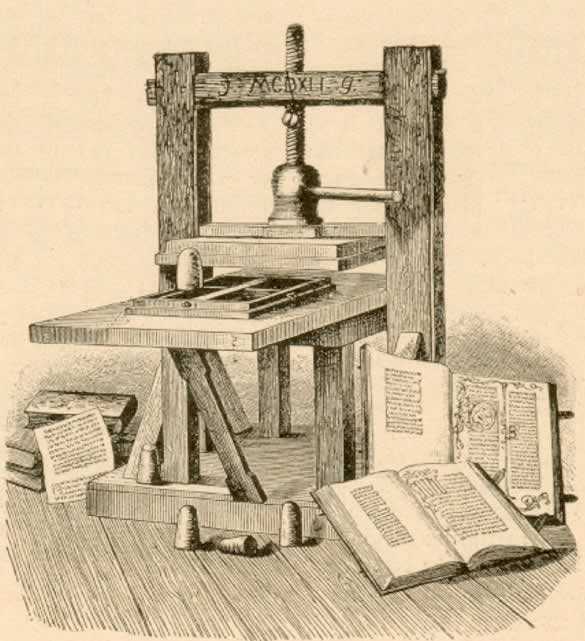
\includegraphics[width=0.7\textwidth]{images/presse} 
\caption[Druckerpresse von Gutenberg \cite{fig:presse}]{Druckerpresse von Gutenberg}
\label{fig:druckerpresse}
\end{figure}

Das Buch wurde zum Massenprodukt und damit zum Katalysator der Wissensgesellschaft die in logischer Konsequenz zur heutigen Informationsgesellschaft f"uhrte.


%%% Local Variables: 
%%% mode: latex
%%% TeX-master: "thesis"
%%% End: 

%% technisch.tex
%% $Id: technisch.tex 61 2012-05-03 13:58:03Z bless $
%%

\chapter{Technische Speicherung}
\label{ch:Technische Speicherung}
%% ==============================  

	%% ==============================
    \section{Elektronische Speicherung}
    %% ==============================
    \label{ch:Technisch:sec:Elektronische Speicherung}
    %% ==============================
	
	Alle Speichermedien die Daten auf Basis von elektronischen Bauelementen speichern sind unter dem Begriff elektronische Speicher zusammengefasst. Heutzutage werden die integrierten Schaltkreise, die zur elektrischen Speicherung notwendig sind fast nur noch mit Silizium realisert. Die einzelnen k"onnen beliebig angesprochen werden, es ist also keine weitere Teilung des Speichers in Sequenzen notwendig. Weiter unterschieden werden elektronische Speichermedien in fl"uchtige Speicher, permanente Speicher und semi-permanente Speicher.
	
        \subsection{Fl"uchtig}
        %% ==============================
        \label{ch:Technisch:sec:Elektronische Speicherung:sub:Fl"uchtig}
        %% ==============================
        
            Ein fl"uchtiger Speicher kann seine Information nur behalten, wenn er an einem Strom liegt, andernfalls verliert er diese Informationen.
				
				\subsubsection{DRAM}
				%% ==============================
				\label{ch:Technisch:sec:Elektronische Speicherung:sub:Fl"uchtig:subsub:DRAM}
				%% ==============================
				
					Beim \glqq Dynamic Random Access Memory\grqq{} handelt es sich um Speicherbausteine, die nach dem Abschalten der angelegten Spannungsversorgung oder zu späten Wiederauffrischung ihren Dateninhalt auf den Speicherzellen verlieren. Der volatile\footnote[4]{fl"uchtig} Speicher wird haupts"achlich in Computern als Arbeitspeicher eingesetzt, man findet ihn aber auch beispielsweise in Druckern oder in Videospielkonsolen.
					\\
					Technisch gesehen speichert ein Kondensator die Daten, also Einsen und Nullen in dem er entweder geladen oder entladen ist. Ein Schalttransistor beschreibt oder liest den Inhalt dann aus.
				
				\subsubsection{SRAM}
				%% ==============================
				\label{ch:Technisch:sec:Elektronische Speicherung:sub:Fl"uchtig:subsub:SRAM}
				%% ==============================
				
					Der \glqq Static Random Access Memory\grqq{} ist wie der DRAM ebenfalls ein Halbleiterspeicher, der volatil ist. Dauerhaft kann er Daten nur speichern, wenn er mit Strom versorgt wird. Der Unterschied zum DRAM ist dabei, dass der Inhalt nicht wiederaufgefrischt werden muss, da SRAM mit Flipflops realisert wird. Ein Flipflop oder auch bistabile Kippstufe kann zwei Zust"ande(Eins oder Null) einnehmen und "uber lange Zeit speichern, allerdings ist die Speicherzelle des SRAM im Vergleich zum DRAM relativ gro"s.
					\\
					Anwendung findet SRAM in Prozessoren als \textit{Cache} oder in Bereichen bei denen der Dateninhalt "uber l"angere Zeit gespeichert werden soll wie beim CMOS-RAM zur Erhaltung von BIOS-Einstellung\footnote[5]{Basic Input Output System} in PCs und Laptops. Zur Aufrechterhaltung der Stromversorung gen"ugt meist eine kleine Pufferbatterie.
					
					todo: l1 cache und l2 cache?
        
        \subsection{Permanent}
        %% ==============================
        \label{ch:Technisch:sec:Elektronische Speicherung:sub:Permanent}
        %% ==============================
        
            Permanenter Speicher beh"alt seine Daten, die einmal in ihm gespeichert oder verdrahtet wurde. Er kann dann nicht mehr ver"andert werden.
			
				\subsubsection{ROM}
				%% ==============================
				\label{ch:Technisch:sec:Elektronische Speicherung:sub:Fl"uchtig:subsub:ROM}
				%% ==============================
				
					Ein typisches Beispiel f"uer permanten Speicher ist der \glqq Read Only Memory \grqq{} – zu Deutsch \textit{Festwertspeicher} oder \textit{Nur-Lese-Speicher}. ROM kann nur einmal beschrieben werden, dann lassen sich die darauf geschriebenen Daten nicht mehr oder nur sehr langsam oder schwer ver"andern. 
					\\
					Die Hauptanwendung ist somit die Verbreitung und Speicherung von Firmware\footnote[6]{Software die spezifisch an Hardware angepasst ist, "ahnlich einem Betriebsystem, aber selten ein Update braucht}. Auch das BIOS eines PCs ist auf einem ROM gespeichert.
					\\
					Klassische Masken-ROM werden so genannt, weil urspr"unglich ROM in der Herstellung mit einer Art Filmnegativ – der \glqq Maske\grqq{} direkt auf den Chip aufbelichtet wird. Das Verfahren ist aber nur in Massenproduktion "okonomisch Sinnvoll, weshalb bald Speicherbausteine entwickelt wurden, die auch nach der Fertigung noch mit Daten bef"ullt werden konnten.
				
				\subsubsection{PROM}
				%% ==============================
				\label{ch:Technisch:sec:Elektronische Speicherung:sub:Fl"uchtig:subsub:PROM}
				%% ==============================
				
					Einer dieser neu entwickelten Speicherbausteine ist das \glqq Programmable Read Only Memory\grqq{}. Diese lassen sich nach der Fertigung genau einmal Programmieren und behalten dann ihren Zustand. Anfangs enthalten alle Speicherzellen eine \glqq 1\grqq{},einzelne Speicherzellen k"onnen dann sp"ater in eine \glqq0 \grqq{} gewandelt werden.
					\\
					Praktisch werden PROMs heute nicht mehr verwendet. 
            
        \subsection{Semi-permanent}
        %% ==============================
        \label{ch:Technisch:sec:Elektronische Speicherung:sub:Semi-permanent}
        %% ==============================
        
            Von semi-permanenten Speichern spricht man, wenn die Daten permanent gespeichert werden, aber im Gegensatz zum permanenten Speicher auch wieder ver"andert werden k"onnen. 
			
				\subsubsection{EPROM}
				%% ==============================
				\label{ch:Technisch:sec:Elektronische Speicherung:sub:Fl"uchtig:subsub:EPROM}
				%% ==============================
					
					Bei der EPROM-Technologie handelt es sich um die Weiterentwicklung von ROM. EPROM steht f"ur \glqq Erasable Programmable Read Only Memory\grqq{} und ist ROM, der aber auch wieder gel"oscht(und damit ver"andert) werden kann. Damit man aber EPROMs programmieren kann, bedarf es spezieller Progammierger"ate – dem \glqq EPROM-Brenner\grqq{}. Mit UV-Licht kann der Speicher dann wieder gel"oscht werden.
					\\
					Weiterhin gibt es noch elektronisch l"oschbaren Speicher EEPROM(\glqq Electrical Erasable Read Only Memory\grqq{}), welches mit Flash-EEPROM EPROM verdr"angt hat.
				
				\subsubsection{Flash-EEPROM}
				%% ==============================
				\label{ch:Technisch:sec:Elektronische Speicherung:sub:Fl"uchtig:subsub:Flash-EEPROM}
				%% ==============================
				
					Dieser elektronisch l"oschbare ROM EEPROM(\glqq Electrical Erasable Read Only Memory\grqq{}) hat den entscheidenen Vorteil, dass er kein spezielles Verfahren braucht um neu beschrieben zu werden; gleichzeitig beh"alt er auf ihm gespeicherte Daten auch ohne eine Spannung aufrecht erhalten zu m"ussen. Ein im Alltag sehr bekannter Begleiter dieses Speicherverfahrens ist der USB-Stick. 
					\\
					Durch seine kompakten Ma"se ist er sehr portabel und die mittlerweile g"angigen Speichergr"o"sen reichen von 2 Gigabyte bis zu 256 GB. Er l"asst sich an jeden USB-Host anschlie"sen, Daten lassen sich so einfach austauschen. 
					\\
					Da die Entwicklung der Flash Speicher erst sp"at begonnen hat, lassen sich heute noch nicht die Speichergr"o"sen von handels"ublichen Festplatten erreichen, doch daf"ur sind sie stromsparender und deutlich praktischer.
				
				\subsubsection{SSD}
				%% ==============================
				\label{ch:Technisch:sec:Elektronische Speicherung:sub:Fl"uchtig:subsub:SSD}
				%% ==============================
				
				%Obwohl die SSD nicht ganz mit der Pyramide vereinbar ist, geh"ort sie trotzdem in die obere Sektion%%eventuell in die einleitung schreiben??
				Die Solid State Drive(SSD) ist ein nichtfl"uchtiger und auf Flash-Technologie basierter Speicher. Er hat keine mechanisch beweglichen Teile mehr wie bei der konventionellen Festplatte. Dadurch vebraucht sie weniger Strom und die Zugriffszeiten sind enorm hoch. H"aufig werden SSDs im 2,5\" Format verkauft, sie sind allerdings nicht an die Normen f"ur optische oder magnetische Speicherplatten gebunden und sind daher z.B. auch als PCI-Steckkarte aufzufinden.
				\\
				Durch die immer weiter sinkenden Preise pro Gigabyte und die unumst"o"slichen Vorteile ist eine dauerfristige Abl"osung von magnetischen Fesplatten durch Solid State Drives zu sehen.
				
				
%% ==============================%% ==============================%% ==============================%% ==============================   		
			
			
			
    %% ==============================
    \section{Magnetische Speicherung}
    %% ==============================
    \label{ch:Technisch:sec:Magnetische Speicherung}
    %% ==============================
    
    Magnetische Speichermedien behalten ihre Informationen, in dem mit Hilfe eines Lese-Schreib-Kopfes Daten auf magnetisierbares Material gebracht werden. Unterschieden wird dann jeweils weiter in nicht rotierende und rotierende Speichermedien. Die nicht rotierenden Speichermedien werden weiter in digitale und analoge Medien unterteilt. Zum ersteren geh"oren Magnetstreifen oder Magnetband. Ein analoges nicht rotierendes Speichermedium ist das Ton- oder Videoband. Die bekannten Festplatten werden zu rotierenden Speichermedien gez"ahlt und sind heute der weit verbreiteste Massenspeicher.

        \subsection{Festplatte}
        %% ==============================
        \label{ch:Technisch:sec:Magnetische Speicherung:sub:Festplatte}
        %% ==============================
        
            Die Festplatte oder das Festplattenlaufwerk speichert Informationen, in dem sie Daten auf die Oberfl"ache einer rotierenden Scheibe schreibt. Die Scheiben sind genau "ubereinander gelagert und drehen sich zur selben Zeit. Die hartmagnetische Beschichtung an der Plattenoberfl"ache wird dann mit den Lese-Schreib-Kopf entweder gelesen oder beschrieben. Auf die Daten kann wahlfrei zugegriffen werden und auch nach dem Ausschalten bleiben die Daten durch Remanenz\footnote[7]{Remanenz ist die zur"uckbleibende Magnetisierung eines magnetischen K"orpers} erhalten. W"ahrend die erste Fesplatte noch eine Tonne wog und nur eine Kapazit"at von 5 Megabyte hatte, haben heutige Festplatten eine Gr"o"se von bis zu 4 Terabyte. Im Gegensatz zu einer SSD k"onnen Festplatten nahezu beliebig oft gel"oscht und neu beschrieben werden.
            \\
            Das Anschlie"sen an einen PC erfolgt mittlerweile entweder intern "uber den Serial ATA-Anschlu"s oder extern "uber USB\footnote[8]{Universal Serial Bus}, Firewire, Thunderbolt oder eSATA. 
    
    
    %% ==============================
    \section{Optische Speicherung}
    %% ==============================
    \label{ch:Technisch:sec:Optische Speicherung}
    %% ==============================
    
        Das optische Speichermedium erh"alt die Daten entweder mechanisch in einem Presswerk(meist kommerziell hergestellte Disks) oder "uber einen Laser(meist private so gennante \glqq gebrannte\grqq{} Disks) in Form von Erh"ohungen(Pits) und Vertiefungen(Lands) auf eine Scheibe. Meistens trifft man bei optischen Speichermedien auf die CD, der DVD oder der Blu-ray Disc. Diese unterscheiden sich in ihrer Speicherkapazit"at, jedoch nicht in ihrer physikalischen Gr"o"se – 8\texttt{"{}} Durchmesser.
        \\
         Die allgemeinen Verkaufszahlen von optischen Speichermedien sind in den letzten Jahren gesunken, da nun zunehmen durch h"ohere Bandbreiten des Internets sich neue Distributionswege er"offnet haben.

        
{%Gruppe auf   
\label{ch:Technisch:sec:Optische SpeicherungM}     
\begin{table}[ht]
\small
\begin{tabular}{|p{3.8cm}|p{3.2cm}|p{3cm}|p{3cm}|}
\hline
~ & CD & DVD & Blu-ray \\ \hline
Kapazit"at & bis zu 900 MB & 4,7 GB (Single Layer)\newline 8,5 GB (Dual Layer)  & 25 GB (Single Layer) bis zu 500 GB (20 Layer) \\  \hline
Lesegeschwindigkeit & 176 KB/s (CD-DA)\newline 150 KB/s (1x) \newline 10800 KB/s (72x) & 1,385 MB/s (1x) & 36 Mbit/s (8x) \\ \hline
Schreibgeschwindigkeit & 150 KB/s (1x)  8400 KB/s (56x) & 1,385 MB/s (1x) & 4,5 MB/s (1x) (DVD 3x) \\ \hline
Gebrauch & Datenspeicher, Audio-CD & Datenspeicher, Video-DVD & Datenspeicher, Video-Blu-ray \\ \hline
Vorstellung & 1981 & 1995 & 2002 \\
\hline
\end{tabular}
\caption{Vergleich optischer Medien}
\label{tab:vlgOptMed}
\end{table}
}%gruppe zu


        \subsection{CD}
        %% ==============================
        \label{ch:Technisch:sec:Optische Speicherung:sub:CD}
        %% ==============================
        
            Die Compact Disk wurde von Phillips und Sony im Jahr 1981 als Speichermedium f"ur Audio(CD-DA\footnote[9]{Compact Disc - Digital Audio}) eingef"uhrt(vgl. Tabelle \ref{tab:vlgOptMed}). Sp"ater erst wurde die CD als CD-ROM zur Datenspeicherung bei Computer benutzt. 
        
        \subsection{DVD}
        %% ==============================
        \label{ch:Technisch:sec:Optische Speicherung:sub:DVD}
        %% ==============================
        
            Die Digital Versatile Disk\footnote[10]{engl. f"ur digitale vielseitige Scheibe} ist der direkte Nachfolger der CD und wurde mit anwachsenden Speicherbedarf n"otig. 
            \\
            Die h"ohere Speicherkapazit"at bei gleichen Durchmesser kommt durch verschiedene Techniken zu Stande. Zum einen wurden die Strahlen des Abtastlasers gek"uerzt und auch die Wellenl"ange wurde k"urzer. Der kleine Laserspot erm"oglichte dann feinere Fl"achen abzutasten und somit mehr Informationen pro Gr"o"seneinheit zu speichern. Au"serdem wurde im Jahr 2004 die Dual Layer DVD vorgestellt, also die \glqq Doppel-Schichten DVD\grqq{}. Somit konnte man doppelt soviele Daten wie auf einer Single Layer DVD speichern. Bis zu 8,5 Gigabyte waren nun m"oglich.
        
        \subsection{Blu-Ray}
        %% ==============================
        \label{ch:Technisch:sec:Optische Speicherung:sub:Blu-Ray}
        %% ==============================
        
            Die Blu-ray Disc Association stellte 2002 die Blu-ray Disc vor. Der Name zielt auf den Abtastlaser ab, der eine violette Farbe hat. Blu\textbf{e} Ray wurde absichtlich falsch geschrieben, um die Registrierung als Namen zu vereinfachen. Die Blu-ray setzte sich 2008 gegen den Konkurrenten HD-DVD durch und fasst schon mit einem Single Layer 25 Gigabyte. Der Markt f"ur hochaufl"osende Filme war damit f"ur den Endverbraucher ge"offnet.
            \\
           



%%% Local Variables: 
%%% mode: latex
%%% TeX-master: "thesis"
%%% End: 

%%% analyse.tex
%% $Id: analyse.tex 61 2012-05-03 13:58:03Z bless $

\chapter{Analyse}
\label{ch:Analyse}
%% ==============================
In diesem Kapitel sollten zun�chst das zu l�sende Problem
sowie die Anforderungen und die Randbedingungen 
einer L�sung\index{L�sung} beschrieben werden (also nochmal
eine pr�zisierte Aufgabenstellung\index{Aufgabenstellung}).

Dann folgt �blicherweise ein �berblick �ber bereits existierende
L�sungen bzw. Ans�tze, die meistens andere Voraussetzungen bzw.
Randbedingungen annehmen.

Bla fasel\ldots

%% ==============================
\section{Anforderungen}
%% ==============================
\label{ch:Analyse:sec:Anforderungen}
Anforderungen und Randbedingungen\index{Randbedingungen} \ldots

%% ==============================
\section{Existierende L�sungsans�tze}
%% ==============================
\label{ch:Analyse:sec:RelatedWork}

Hier kommt eine ausf�hrliche Diskussion
von "`Related Work"'.

Bla fasel\ldots

%% ==============================
\section{Weiterer Abschnitt}
%% ==============================
\label{ch:Analyse:sec:Abschnitt}

Bla fasel\ldots hat auch schon \cite{TB2000} gesagt und
\cite{TB98,JSAC96,qosr} sollte man mal gelesen haben.
Abbildung~\ref{fig:test} auf S.~\pageref{fig:test} sollte man
sich mal anschauen.

Blindtext Blindtext Blindtext Blindtext Blindtext Blindtext Blindtext
Blindtext Blindtext Blindtext Blindtext Blindtext Blindtext Blindtext
Blindtext Blindtext Blindtext Blindtext Blindtext Blindtext Blindtext
Blindtext Blindtext Blindtext Blindtext Blindtext Blindtext Blindtext
Blindtext Blindtext Blindtext Blindtext Blindtext Blindtext Blindtext
Blindtext Blindtext Blindtext Blindtext Blindtext Blindtext Blindtext
Blindtext Blindtext Blindtext Blindtext Blindtext Blindtext Blindtext
Blindtext Blindtext Blindtext Blindtext Blindtext Blindtext Blindtext
Blindtext Blindtext Blindtext Blindtext Blindtext Blindtext Blindtext

Blindtext Blindtext Blindtext Blindtext Blindtext Blindtext Blindtext
Blindtext Blindtext Blindtext Blindtext Blindtext Blindtext Blindtext
Blindtext Blindtext Blindtext Blindtext Blindtext Blindtext Blindtext
Blindtext Blindtext Blindtext Blindtext Blindtext Blindtext Blindtext
Blindtext Blindtext Blindtext Blindtext Blindtext Blindtext Blindtext
Blindtext Blindtext Blindtext Blindtext Blindtext Blindtext Blindtext
Blindtext Blindtext Blindtext Blindtext Blindtext Blindtext Blindtext
Blindtext Blindtext Blindtext Blindtext Blindtext Blindtext Blindtext
Blindtext Blindtext Blindtext Blindtext Blindtext Blindtext Blindtext
Blindtext Blindtext Blindtext Blindtext Blindtext Blindtext Blindtext
Blindtext Blindtext Blindtext Blindtext Blindtext Blindtext Blindtext
Blindtext Blindtext Blindtext Blindtext Blindtext Blindtext Blindtext
Blindtext Blindtext Blindtext Blindtext Blindtext Blindtext Blindtext

Blindtext Blindtext Blindtext Blindtext Blindtext Blindtext Blindtext
Blindtext Blindtext Blindtext Blindtext Blindtext Blindtext Blindtext
Blindtext Blindtext Blindtext Blindtext Blindtext Blindtext Blindtext
Blindtext Blindtext Blindtext Blindtext Blindtext Blindtext Blindtext
Blindtext Blindtext Blindtext Blindtext Blindtext Blindtext Blindtext
Blindtext Blindtext Blindtext Blindtext Blindtext Blindtext Blindtext
Blindtext Blindtext Blindtext Blindtext Blindtext Blindtext Blindtext
Blindtext Blindtext Blindtext Blindtext Blindtext Blindtext Blindtext
Blindtext Blindtext Blindtext Blindtext Blindtext Blindtext Blindtext
Blindtext Blindtext Blindtext Blindtext Blindtext Blindtext Blindtext

Blindtext Blindtext Blindtext Blindtext Blindtext Blindtext Blindtext
Blindtext Blindtext Blindtext Blindtext Blindtext Blindtext Blindtext
Blindtext Blindtext Blindtext Blindtext Blindtext Blindtext Blindtext
Blindtext Blindtext Blindtext Blindtext Blindtext Blindtext Blindtext
Blindtext Blindtext Blindtext Blindtext Blindtext Blindtext Blindtext
Blindtext Blindtext Blindtext Blindtext Blindtext Blindtext Blindtext
Blindtext Blindtext Blindtext Blindtext Blindtext Blindtext Blindtext
Blindtext Blindtext Blindtext\index{Blindtext} Blindtext Blindtext Blindtext Blindtext

\begin{figure}[!htbp]
  \centering
  \fbox{\parbox{0.8\textwidth}{
  Abbildungen sollten m�glichst als EPS (Encapsulated Postscript) 
  bzw. PDF eingebunden werden.
  Zur Erzeugung sauberer EPS-Dateien empfiehlt sich das Tool \texttt{ps2eps}
  zur Nachbearbeitung von Postscript-Dateien. Mit \texttt{epstopdf} kann
  dann eine PDF-Datei zum Einbinden erzeugt werden.}}
  \caption{Testabbildung}
  \label{fig:test}
\end{figure}

Blindtext Blindtext Blindtext Blindtext Blindtext Blindtext Blindtext
Blindtext Blindtext Blindtext Blindtext Blindtext Blindtext Blindtext
Blindtext Blindtext Blindtext Blindtext Blindtext Blindtext Blindtext
Blindtext Blindtext Blindtext Blindtext Blindtext Blindtext Blindtext
Blindtext Blindtext Blindtext Blindtext Blindtext Blindtext Blindtext
Blindtext Blindtext Blindtext Blindtext Blindtext Blindtext Blindtext
Blindtext Blindtext Blindtext Blindtext Blindtext Blindtext Blindtext

Blindtext Blindtext Blindtext Blindtext Blindtext Blindtext Blindtext
Blindtext Blindtext Blindtext Blindtext Blindtext Blindtext Blindtext
Blindtext Blindtext Blindtext Blindtext Blindtext Blindtext Blindtext

Blindtext Blindtext Blindtext Blindtext Blindtext Blindtext Blindtext
Blindtext Blindtext Blindtext Blindtext Blindtext Blindtext Blindtext
Blindtext Blindtext Blindtext Blindtext Blindtext Blindtext Blindtext
Blindtext Blindtext Blindtext Blindtext Blindtext Blindtext Blindtext
Blindtext Blindtext Blindtext Blindtext Blindtext Blindtext Blindtext
Blindtext Blindtext Blindtext Blindtext Blindtext Blindtext Blindtext

Blindtext Blindtext Blindtext Blindtext Blindtext Blindtext Blindtext
Blindtext Blindtext Blindtext Blindtext Blindtext Blindtext Blindtext
Blindtext Blindtext Blindtext Blindtext Blindtext Blindtext Blindtext
Blindtext Blindtext Blindtext Blindtext Blindtext Blindtext Blindtext
Blindtext Blindtext Blindtext Blindtext Blindtext Blindtext Blindtext
Blindtext Blindtext Blindtext Blindtext Blindtext Blindtext Blindtext
Blindtext Blindtext Blindtext Blindtext Blindtext Blindtext Blindtext
Blindtext Blindtext Blindtext Blindtext Blindtext Blindtext Blindtext
Blindtext Blindtext Blindtext Blindtext Blindtext Blindtext Blindtext
Blindtext Blindtext Blindtext Blindtext Blindtext Blindtext Blindtext
Blindtext Blindtext Blindtext Blindtext Blindtext Blindtext Blindtext
Blindtext Blindtext Blindtext Blindtext Blindtext Blindtext Blindtext
Blindtext Blindtext Blindtext Blindtext Blindtext Blindtext Blindtext
Blindtext Blindtext Blindtext Blindtext Blindtext Blindtext Blindtext

Blindtext Blindtext Blindtext Blindtext Blindtext Blindtext Blindtext
Blindtext Blindtext Blindtext Blindtext Blindtext Blindtext Blindtext
Blindtext Blindtext Blindtext Blindtext Blindtext Blindtext Blindtext
Blindtext Blindtext Blindtext Blindtext Blindtext Blindtext Blindtext
Blindtext Blindtext Blindtext Blindtext Blindtext Blindtext Blindtext
Blindtext Blindtext Blindtext Blindtext Blindtext Blindtext Blindtext
Blindtext Blindtext Blindtext Blindtext Blindtext Blindtext Blindtext
Blindtext Blindtext Blindtext Blindtext Blindtext Blindtext Blindtext
Blindtext Blindtext Blindtext Blindtext Blindtext Blindtext Blindtext
Blindtext Blindtext Blindtext Blindtext Blindtext Blindtext Blindtext
Blindtext Blindtext Blindtext Blindtext Blindtext Blindtext Blindtext
%% ==============================
\section{Zusammenfassung}
%% ==============================
\label{ch:Analyse:sec:zusammenfassung}

Am Ende sollten ggf. die wichtigsten Ergebnisse nochmal in \emph{einem}
kurzen Absatz zusammengefasst werden.

%%% Local Variables: 
%%% mode: latex
%%% TeX-master: "thesis"
%%% End: 
     % Analyse
%%% entwurf.tex
%% $Id: entwurf.tex 61 2012-05-03 13:58:03Z bless $
%%

\chapter{Entwurf}
\label{ch:Entwurf}
%% ==============================
In diesem Kapitel erfolgt die ausf�hrliche Beschreibung des eigenen
L�sungsansatzes. Dabei sollten L�sungsalternativen diskutiert und
Entwurfsentscheidungen dargelegt werden.


Bla fasel\ldots

%% ==============================
\section{Abschnitt 1}
%% ==============================
\label{ch:Entwurf:sec:Abschnitt1}

Bla fasel\ldots

%% ==============================
\section{Abschnitt 2}
%% ==============================
\label{ch:Entwurf:sec:Abschnitt2}

Bla fasel\ldots

Blindtext Blindtext Blindtext Blindtext Blindtext Blindtext Blindtext
Blindtext Blindtext Blindtext Blindtext Blindtext Blindtext Blindtext
Blindtext Blindtext Blindtext Blindtext Blindtext Blindtext Blindtext
Blindtext Blindtext Blindtext Blindtext Blindtext Blindtext Blindtext
Blindtext Blindtext Blindtext Blindtext Blindtext Blindtext Blindtext
Blindtext Blindtext Blindtext Blindtext Blindtext Blindtext Blindtext
Blindtext Blindtext Blindtext Blindtext Blindtext Blindtext Blindtext
Blindtext Blindtext Blindtext Blindtext Blindtext Blindtext Blindtext
Blindtext Blindtext Blindtext Blindtext Blindtext Blindtext Blindtext
Blindtext Blindtext Blindtext Blindtext Blindtext Blindtext Blindtext
Blindtext Blindtext Blindtext Blindtext Blindtext Blindtext Blindtext
Blindtext Blindtext Blindtext Blindtext Blindtext Blindtext Blindtext
Blindtext Blindtext Blindtext Blindtext Blindtext Blindtext Blindtext
Blindtext Blindtext Blindtext Blindtext Blindtext Blindtext Blindtext
Blindtext Blindtext Blindtext Blindtext Blindtext Blindtext Blindtext
Blindtext Blindtext Blindtext Blindtext Blindtext Blindtext Blindtext
Blindtext Blindtext Blindtext Blindtext Blindtext Blindtext Blindtext

Blindtext Blindtext Blindtext Blindtext Blindtext Blindtext Blindtext
Blindtext Blindtext Blindtext Blindtext Blindtext Blindtext Blindtext
Blindtext Blindtext Blindtext Blindtext Blindtext Blindtext Blindtext
Blindtext Blindtext Blindtext Blindtext Blindtext Blindtext Blindtext
Blindtext Blindtext Blindtext Blindtext Blindtext Blindtext Blindtext
Blindtext Blindtext Blindtext Blindtext Blindtext Blindtext Blindtext
Blindtext Blindtext Blindtext Blindtext Blindtext Blindtext Blindtext
Blindtext Blindtext Blindtext Blindtext Blindtext Blindtext Blindtext
Blindtext Blindtext Blindtext Blindtext Blindtext Blindtext Blindtext
Blindtext Blindtext Blindtext Blindtext Blindtext Blindtext Blindtext
Blindtext Blindtext Blindtext Blindtext Blindtext Blindtext Blindtext
Blindtext Blindtext Blindtext Blindtext Blindtext Blindtext Blindtext
Blindtext Blindtext Blindtext Blindtext Blindtext Blindtext Blindtext
Blindtext Blindtext Blindtext Blindtext Blindtext Blindtext Blindtext
Blindtext Blindtext Blindtext Blindtext Blindtext Blindtext Blindtext
Blindtext Blindtext Blindtext Blindtext Blindtext Blindtext Blindtext
Blindtext Blindtext Blindtext Blindtext Blindtext Blindtext Blindtext
Blindtext Blindtext Blindtext Blindtext Blindtext Blindtext Blindtext
Blindtext Blindtext Blindtext Blindtext Blindtext Blindtext Blindtext
Blindtext Blindtext Blindtext Blindtext Blindtext Blindtext Blindtext

Blindtext Blindtext Blindtext Blindtext Blindtext Blindtext Blindtext
Blindtext Blindtext Blindtext Blindtext Blindtext Blindtext Blindtext
Blindtext Blindtext Blindtext Blindtext Blindtext Blindtext Blindtext
Blindtext Blindtext Blindtext Blindtext Blindtext Blindtext Blindtext
Blindtext Blindtext Blindtext Blindtext Blindtext Blindtext Blindtext
Blindtext Blindtext Blindtext Blindtext Blindtext Blindtext Blindtext
Blindtext Blindtext Blindtext Blindtext Blindtext Blindtext Blindtext
Blindtext Blindtext Blindtext Blindtext Blindtext Blindtext Blindtext
Blindtext Blindtext Blindtext Blindtext Blindtext Blindtext Blindtext
Blindtext Blindtext Blindtext Blindtext Blindtext Blindtext Blindtext
Blindtext Blindtext Blindtext Blindtext Blindtext Blindtext Blindtext
Blindtext Blindtext Blindtext Blindtext Blindtext Blindtext Blindtext
Blindtext Blindtext Blindtext Blindtext Blindtext Blindtext Blindtext
Blindtext Blindtext Blindtext Blindtext Blindtext Blindtext Blindtext
Blindtext Blindtext Blindtext Blindtext Blindtext Blindtext Blindtext

Blindtext Blindtext Blindtext Blindtext Blindtext Blindtext Blindtext
Blindtext Blindtext Blindtext Blindtext Blindtext Blindtext Blindtext
Blindtext Blindtext Blindtext Blindtext Blindtext Blindtext Blindtext
Blindtext Blindtext Blindtext Blindtext Blindtext Blindtext Blindtext
Blindtext Blindtext Blindtext Blindtext Blindtext Blindtext Blindtext
Blindtext Blindtext Blindtext Blindtext Blindtext Blindtext Blindtext
Blindtext Blindtext Blindtext Blindtext Blindtext Blindtext Blindtext
Blindtext Blindtext Blindtext Blindtext Blindtext Blindtext Blindtext
Blindtext Blindtext Blindtext Blindtext Blindtext Blindtext Blindtext
Blindtext Blindtext Blindtext Blindtext Blindtext Blindtext Blindtext
Blindtext Blindtext Blindtext Blindtext Blindtext Blindtext Blindtext
Blindtext Blindtext Blindtext Blindtext Blindtext Blindtext Blindtext
Blindtext Blindtext Blindtext Blindtext Blindtext Blindtext Blindtext
Blindtext Blindtext Blindtext Blindtext Blindtext Blindtext Blindtext
Blindtext Blindtext Blindtext Blindtext Blindtext Blindtext Blindtext
Blindtext Blindtext Blindtext Blindtext Blindtext Blindtext Blindtext

Blindtext Blindtext Blindtext Blindtext Blindtext Blindtext Blindtext
Blindtext Blindtext Blindtext Blindtext Blindtext Blindtext Blindtext
Blindtext Blindtext Blindtext Blindtext Blindtext Blindtext Blindtext
Blindtext Blindtext Blindtext Blindtext Blindtext Blindtext Blindtext
Blindtext Blindtext Blindtext Blindtext Blindtext Blindtext Blindtext
Blindtext Blindtext Blindtext Blindtext Blindtext Blindtext Blindtext
Blindtext Blindtext Blindtext Blindtext Blindtext Blindtext Blindtext
Blindtext Blindtext Blindtext Blindtext Blindtext Blindtext Blindtext
Blindtext Blindtext Blindtext Blindtext Blindtext Blindtext Blindtext
Blindtext Blindtext Blindtext Blindtext Blindtext Blindtext Blindtext
Blindtext Blindtext Blindtext Blindtext Blindtext Blindtext Blindtext
Blindtext Blindtext Blindtext Blindtext Blindtext Blindtext Blindtext
Blindtext Blindtext Blindtext Blindtext Blindtext Blindtext Blindtext

%% ==============================
\section{Zusammenfassung}
%% ==============================
\label{ch:Entwurf:sec:zusammenfassung}

Am Ende sollten ggf. die wichtigsten Ergebnisse nochmal in \emph{einem}
kurzen Absatz zusammengefasst werden.

%%% Local Variables: 
%%% mode: latex
%%% TeX-master: "thesis"
%%% End: 
     % Entwurf
%%% implemen.tex
%% $Id: implemen.tex 61 2012-05-03 13:58:03Z bless $
%%
% !TEX root = thesis.tex

\chapter{Implementierung}
\label{ch:Implementierung}
%% ==============================
Bla fasel\ldots

%% ==============================
\section{Abschnitt 1}
%% ==============================
\label{ch:Implementierung:sec:Abschnitt1}

Bla fasel\ldots

%% ==============================
\section{Abschnitt 2}
%% ==============================
\label{ch:Implementierung:sec:Abschnitt2}

Bla fasel\ldots

%%% Local Variables: 
%%% mode: latex
%%% TeX-master: "thesis"
%%% End: 
    % Implementierung
%%% eval.tex
%% $Id: eval.tex 61 2012-05-03 13:58:03Z bless $
% !TEX root = thesis.tex

\chapter{Evaluierung}
\label{ch:Evaluierung}
%% ==============================
Hier kommt der Nachweis, dass das in Kapitel~\ref{ch:Entwurf}
entworfene Konzept auch funktioniert. Leistungsmessungen einer
Implementierung werden auch immer gerne gesehen.

Bla fasel\ldots

%% ==============================
\section{Abschnitt 1}
%% ==============================
\label{ch:Evaluierung:sec:Abschnitt1}

Bla fasel\ldots

%% ==============================
\section{Abschnitt 2}
%% ==============================
\label{ch:Evaluierung:sec:Abschnitt2}

Bla fasel\ldots

%% ==============================
\section{Zusammenfassung}
%% ==============================
\label{ch:Evaluierung:sec:zusammenfassung}

Am Ende sollten ggf. die wichtigsten Ergebnisse nochmal in \emph{einem}
kurzen Absatz zusammengefasst werden.

%%% Local Variables: 
%%% mode: latex
%%% TeX-master: "thesis"
%%% End: 
        % Evaluierung
%% zusammenf.tex
%% $Id: zusammenf.tex 61 2012-05-03 13:58:03Z bless $
%%

\chapter{Zusammenfassung und Ausblick}
\label{ch:Zusammenfassung}
%% ==============================
Zusammenfassend l"asst sich also sagen, dass es viele M"oglichkeiten heute gibt, Daten zu speichern. Die einen sind praktischer, die anderen etwas unpraktischer.
Der meist genutzte Massenspeicher ist im Moment wohl die Festplatte, seine Entwicklung war rasant – "ahnlich dem \textit{Mooreschen Gesetz} zeigt sie einen ann"ahernd exponentiellen Verlauf wie die Abbildung \ref{fig:kapazit} zeigt. Alle 16 Monate etwa, verdoppelt sich damit die Speicherkapazit"at
\begin{figure}[ht]
				\centering
				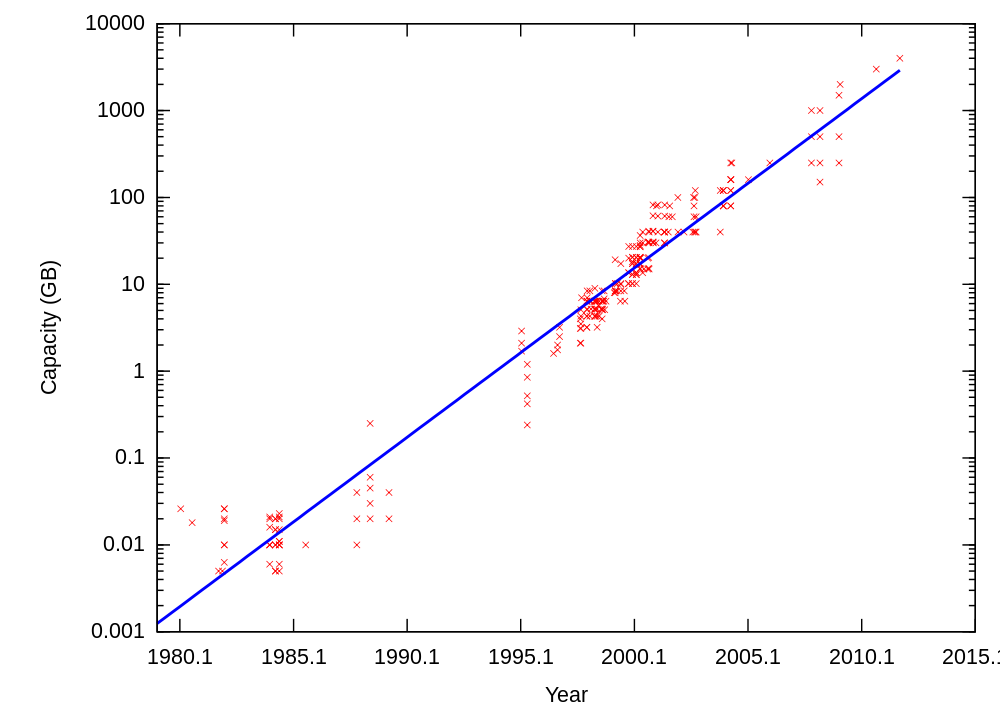
\includegraphics[width=0.7\textwidth]{images/kapazit} 
				\caption[Entwicklung Speicherkapazit"at Fesplatte in halblogarithmischer Skalierung \cite{fig:kapazit}]{Entwicklung Speicherkapazit"at Fesplatte in halblogarithmischer Skalierung}
				\label{fig:kapazit}
				\end{figure}
\\
Auch die Rohstoffverknappung k"onnte den Speicherhunger behindern, wie die Flutkatastrophe Ende 2011 in Thailand zeigte. Die Preise f"ur Festplatten stiegen darauf hin, da nahezu alle Festplatten der Marktriesen dort produziert wurden.
\\
Doch irgendwann wird die physikalische Grenze erreicht werden.
\\
Das Ziel ist 1 Bit = 1 Atom, das Speichern auf atomarer Ebene. Im Januar 2012 konnten die Forscher des IBM Almaden Research Centers zusammen mit Forschern der Max-Planck-Gesellschaft den kleinsten Speicher der Welt bauen. Sie haben es geschafft einen 12 Atom Speicher zu bauen, allerdings ist dieser nur bei -268 Grad zuverl"assig. Bis er bei Raumtemperaturen funktioniert und Marktreif ist, wird es wohl noch einige Zeit dauern.\cite{heise:ibm} 
\\
Dann wird es aber wohl m"oglich sein die gesamte Weltliteratur auf einen Speicher von der Gr"o"se einer Briefmarke zu speichern. 

%%% Local Variables: 
%%% mode: latex
%%% TeX-master: "thesis"
%%% End: 
   % Zusammenfassung und Ausblick

%% ++++++++++++++++++++++++++++++++++++++++++
%% Anhang
%% ++++++++++++++++++++++++++++++++++++++++++

\appendix
%\include{anhang_a}
%\include{anhang_b}

%% ++++++++++++++++++++++++++++++++++++++++++
%% Literatur
%% ++++++++++++++++++++++++++++++++++++++++++
%  mit dem Befehl \nocite werden auch nicht 
%  zitierte Referenzen abgedruckt
\cleardoublepage
\phantomsection
\addcontentsline{toc}{chapter}{\bibname}
%%

\nocite{*} % nur angeben, wenn auch nicht im Text zitierte Quellen 
           % erscheinen sollen
%\bibliographystyle{itmabbrv} % mit abgekürzten Vornamen der Autoren
%\bibliographystyle{gerplain} % abbrvnat unsrtnat
% spezielle Zitierstile: Labels mit vier Buchstaben und Jahreszahl
%\bibliographystyle{itmalpha}  % ausgeschriebene Vornamen der Autoren
\bibliographystyle{ieeetr} 
\bibliography{thesis}

\listoffigures
\listoftables
%% ++++++++++++++++++++++++++++++++++++++++++
%% Index
%% ++++++++++++++++++++++++++++++++++++++++++
\ifnotdraft{
\cleardoublepage
\phantomsection
\printindex            % Index, Stichwortverzeichnis
}
\end{document}
%% end of file
